\documentclass{myproc}
%\addtolength{\topmargin}{-2cm}
%\addtolength{\textheight}{2cm}
\usepackage{mathptm,mydef}
\usepackage{graphicx}
\DeclareGraphicsExtensions{.png,.jpg}
%\usepackage{courier}
\usepackage{epsfig}
\usepackage{alltt}
\usepackage[T1]{fontenc}
\renewcommand{\ttdefault}{txtt}
\usepackage[all]{xy}
%\usepackage{MinionPro}

\usepackage{hyperref}
\hypersetup{
    colorlinks, 
    citecolor=black, 
    filecolor=black, 
    linkcolor=blue, 
    urlcolor=black
}

\begin{document}
\small


\begin{center}
{\large\bf Electric Imp: Overview}
\end{center}


\vspace*{1cm}

\tableofcontents

\section{Overview}
\subsection{Event-driven programming}
\bit
\w \bb{Device code}: Device (code on Device) reacts to Agent (code on cloud)
\begin{alltt}
  // on reception of notification headed 
  // "text_to_display" from the agent, 
  // call "led_matrix_print"
  \textcolor{red2}{agent.on("text_to_disiplay", led_matrix_print);}

  function led_matrix_print(message_to_display) \{
    display_line(message_to_display);
    \textcolor{red2}{agent.send("message_displayed", true);}
  \}
\end{alltt}
\w \bb{Agent code}: Agent (code on cloud) reacts to Device (code on Device)
\begin{alltt}
  \textcolor{blue2}{// HTTP request handler registration}
  \textbf{\textcolor{blue2}{http.onrequest(request_handler);}}

  function request_handler(request, response) \{
    try \{
        if ("message" in request.query) 
          \textcolor{red2}{device.send("text_to_display", 
                      request.query.message);}
    \} 
    catch (ex) \{
        device.send("error_to_display", 
                    "Internal Server Error: " 
                    + ex);
    \}
  \}
\end{alltt}
\w \bb{Timer event}
\begin{alltt}
function loop() \{
    // Gets integer from imp's light sensor, 
    // converts it to string and relays via UART
    local current_light = hardware.lightlevel();
    uart57.write("Current light level is: " + 
                 current_light);

    // Set the imp to check again in one second
    imp.wakeup(1.0, loop);
\}
\end{alltt}
\eit

\subsection{Interactive imp}
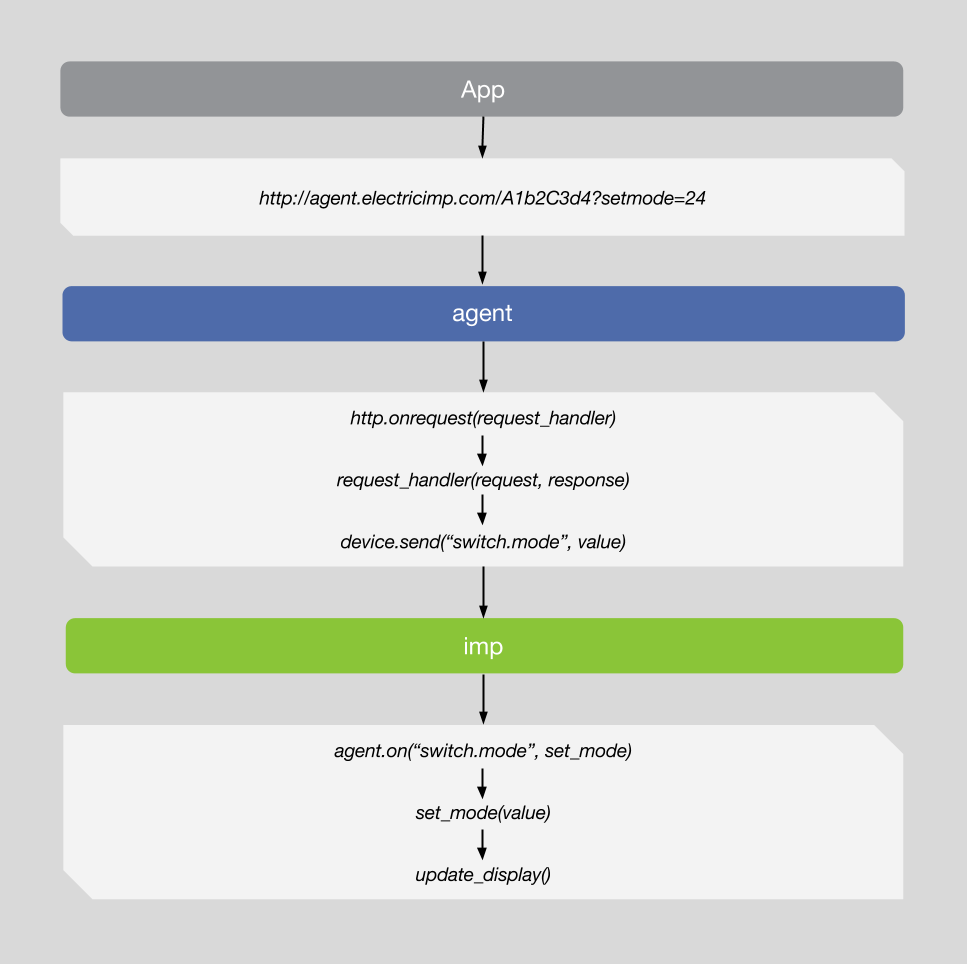
\includegraphics[width=9cm]{pics/interactive}
\bit
\w \textcolor{green2}{managing communication between \bb{app} (U/I),
  \bb{agent} (reactor) and \bb{device}}

\eit


\section{Objects}
\subsection{Overview}
\bit
\w \bb{object}: software construct that combines data (called ``properties'')
and functions (Called ``methods'')
\eit
\subsection{The {\tt{}hardware} object}
The \bb{hardware} object represents an imp's IO peripherals and is used to
control or monitor the hardware in the impee – the device operated by either
an imp card (imp001) or a solder-down imp module (imp002, imp003/Murata
LBWA1ZV1CD). 

The hardware object has the following member methods:
\bit
\w \textcolor{blue2}{\tt{}hardware.getdeviceid()}: returns the
\textcolor{red2}{device's unique ID} as a string 
\w \textcolor{blue2}{\tt{}hardware.lightlevel()}: reads the imp's light-level
sensor 
\w \textcolor{blue2}{\tt{}hardware.micros()}: returns current value of a
free-running microsecond timer 
\w \textcolor{blue2}{\tt{}hardware.millis()}: returns current value of a
free-running millisecond timer 
\w \textcolor{blue2}{\tt{}hardware.voltage()}: returns the imp power supply
voltage 
\w \textcolor{blue2}{\tt{}hardware.wakereason()}: returns the reason the imp
woke up 
\eit
The hardware object also has the following deprecated member methods, which should not be used in new code, but are documented here as an aid to understanding and migrating old code:
\bit
\w \textcolor{blue2}{\tt{}hardware.configure(const,...)}: deprecated and inflexible way to configure the hardware
\w \textcolor{blue2}{\tt{}hardware.getimpeeid()}: returns the device's unique ID as a string
\eit


%\pagebreak

\end{document}
